For all 16 data sets, each of which captures a full minute of oscillation, a value of the decay coefficient $\tau$ is optimized to fit the behaviour of the pendulum. In most cases, the resulting decay coefficient allows the optimized functional fit of the form Eq.(\ref{theta equation}) to perfectly decay alongside of the envelope of the recorded data. This is displayed exquisitely in Figures \ref{exponential_decay1} and \ref{exponential_decay2}, particularly the former of these which carries a goodness of fit estimation of $\chi^2 = 1.35$ and the envelope of which decays by a factor of (over) $1/e$ of its initial value; this objectively proves the exponential decay in the angular amplitude of the mass over time.  With that being said, a few of the functional fits did not result in optimal or expected behaviour. Examples of such fits are included in Figures \ref{P5} and \ref{P6} which clearly indicate that the functional form decays far faster than the collected data itself. This data, however, was taken with initial angular amplitudes of $\theta_0 = 0.68$ and $\theta_0 = 1.02$ respectively; relatively large angles for which the approximation that $\sin\theta\approx \theta$ used to obtain Eq.(\ref{theta equation}) itself becomes increasingly crude. These are examples where the small angle approximation fails; the level at which this approximation remains valid is discussed in further detail below.\\[0.10cm]

In an effort to estimate the \emph{efficiency} of the pendulum, the ratio of the decay coefficient to the period of oscillation is computed for the various combinations of the independent variables. The value of all such ratios are included in Table \ref{decay coeff table} in the appendix, and take on an average value of 108.02 (note that this value is a ratio of values of the same units; the ratio is unitless). If only the cases where the small angle approximation is valid are considered, this ratio takes on an average value of 119.77. These large values indicate a high level of efficiency within the system. \\[0.10cm]

Naturally, the relationship between the independent variables $\ell, m, \theta_0$ and the decay coefficient $\tau$ are of interest. Figure \ref{length_tau} plots the decay coefficient for each length of pendulum, while leaving $m = 0.1\text{kg}$ and $\theta_0 = 0.22\text{rads}$ fixed, alongside two possible functional forms: one linear and one (increasing) quadratic form. Both of these fits provide decent correlation between the length of the pendulum and the decay coefficient, taking on goodness of fit estimations of $\chi^2 = 3.14$ and $\chi^2 = 2.42$ respectively. Since the quadratic form has a better goodness of fit estimation, it follows that the most likely correlation between $\ell$ and $\tau$ is given by
\begin{equation} \label{eq: length_vs_tau}
    \tau(\ell) = \left(2935.98 [\text{s}/\text{m}^2]\right) \ell^2 + \left(6.76 [\text{s}/\text{m}]\right)\ell + 45.79\text{s}
\end{equation}
 Residual plots of the collected data against \emph{both} fits are included in Figures \ref{length_tau_residual1} and \ref{length_tau_residual2}. In a similar vein, Figure \ref{mass_tau} plots the decay coefficients for each value of the mass of the pendulum, while leaving $L = 0.10\text{m}$ and $\theta_0 = 0.22\text{rads}$ fixed. This data is plotted alongside two separately optimized functional forms: one linear form and one logarithmic form, each containing additive constants. The ladder of these plots approximates the data spectacularly having an estimated goodness of fit of $\chi^2 = 1.27$. Since the linear fit fails to obtain a goodness of fit closer to 1, it follows that the most likely correlation between $m$ and $\tau$ is given by
 \begin{equation}\label{eq: mass_vs_tau}
     \tau(m) = \left(38.90\text{s}\right)\log(m/(1\text{kg})) + 167.61\text{s}
 \end{equation}
 \vspace{-0.75cm}
\centering\quad Pendulum Length Versus Decay Coefficient\flushleft
\begin{figure}[H]
    \centerline{\includegraphics[scale=0.55]{Plots/length_vs_tau.png}}
    \caption{\small{A plot of the various decay coefficients for the data with fixed mass $m = 0.1\text{kg}$ and initial angular amplitude $\theta_0 = 0.22\text{rads}$. This data is plotted alongside both a quadratic and linear fits, the form of each being printed onto the image, along with their respective goodness of fit estimations.}}
    \label{length_tau}
\end{figure}

Figure \ref{mass_tau} is accompanied by residual plots for \emph{both} of the aforementioned functional forms given in Figures \ref{mass_tau_residual1} and \ref{mass_tau_residual2} in the appendix. Finally, Figure \ref{amplitude_tau} plots the approximated decay coefficient for each value of the initial angular amplitude while leaving $L = 0.10\text{m}$ and $m = 0.10\text{kg}$ fixed. These data points are plotted alongside two optimized functional forms: one linear and one quadratic (both of which are decreasing on the domain of interest). 


\begin{figure}[H]
\centering
\begin{subfigure}[t]{0.5\textwidth}
  \centering
  \includegraphics[width=1\textwidth]{Plots/masses_vs_tau.png}
  \caption{\small{Pendulum mass versus decay constant.}}
  \label{mass_tau}
\end{subfigure}%
\begin{subfigure}[t]{.5\textwidth}
  \centering
  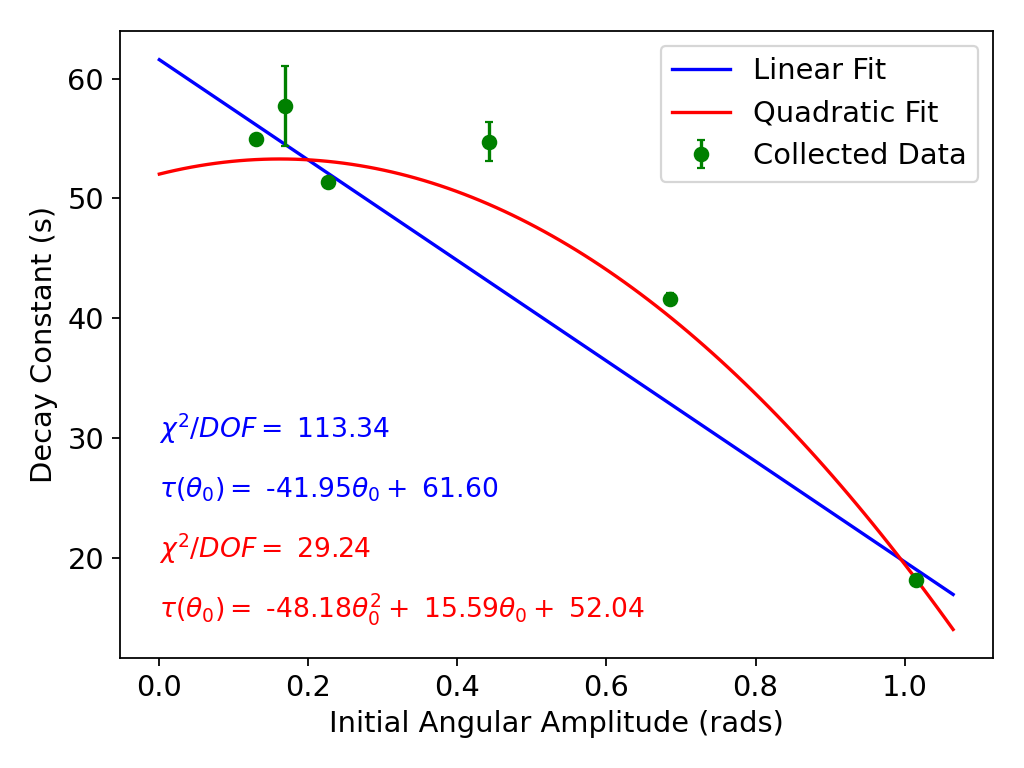
\includegraphics[width=\textwidth]{Plots/theta_vs_tau.png}
  \caption{\small{Pendulum initial angular amplitude versus decay constant}}
  \label{amplitude_tau}
\end{subfigure}
\caption{\small{Plots summarizing the estimated decay constants against the mass of the pendulum and the initial angular amplitude of the data sets respectively. These plots are included with goodness of fit estimations, as well as two possible functional forms each. The data in Figure \ref{mass_tau} is plotted with a linear fit and a logarithmic fit, the ladder of which producing the between goodness of fit estimation. The data in Figure \ref{amplitude_tau} is plotted with a linear fit and a quadratic fit, the ladder of which producing the between goodness of fit estimation.}}
\end{figure}

Admittedly, the goodness of fits for both of these forms are extremely high, indicating a poor correlation. This is likely attributable to a lack of a sufficient number of data points as well as human error. With that being said, the quadratic fit better correlates the two variables, taking on a goodness of fit estimation of $\chi^2 = 29.24$ and has the form given by
\begin{equation} \label{eq: theta_vs_tau}
    \tau(\theta_0) = \left(-41.18[\text{s}/\text{rads}^2]\right)\theta_0^2 + \left(15.59[\text{s}/\text{rads}]\right)\theta_0 + 52.04\text{s}
\end{equation}
Likewise to the above discussions, Figure \ref{amplitude_tau} is accompanied by residual plots for both the optimized forms are given in Figures \ref{theta_tau_residual1} and \ref{theta_tau_residual2}. Note that each of the coefficients in each of the above expression (namely Eqs.(\ref{eq: length_vs_tau}) - (\ref{eq: theta_vs_tau})) carry an uncertainty value which is propagated by the covariance matrix produced by \texttt{curve\_fit}, however their values are not included as it is beyond the focus of this report.\\[0.20cm]
